\documentclass[11pt, oneside]{article}   	% use "amsart" instead of "article" for AMSLaTeX format
\usepackage{geometry}                		% See geometry.pdf to learn the layout options. There are lots.
\geometry{letterpaper}                   		% ... or a4paper or a5paper or ... 
%\geometry{landscape}                		% Activate for rotated page geometry
%\usepackage[parfill]{parskip}    		% Activate to begin paragraphs with an empty line rather than an indent
\usepackage{graphicx}				% Use pdf, png, jpg, or eps§ with pdflatex; use eps in DVI mode
								% TeX will automatically convert eps --> pdf in pdflatex		
\usepackage{amssymb}

%SetFonts

%SetFonts


\title{Comparing Dot Dirichlet To NK}
\author{Adrian Apaza}
%\date{}							% Activate to display a given date or no date

\begin{document}
\maketitle
%\section{}
%\subsection{}

The Dot Dirichlet Model differs crucially from the Standard NK when we observe the Local Optima Networks. LONs are clustered networks showing what local maxima are reachable from each other when a step size of two may be taken from one maxima; they illustrate how many optima are in the same basin of attraction and reachable to each-other. We notice that the Dot Dirichlet models will, for a given number of local maxima, contain fewer clusters - thus one local optimum may be reached from another. We see that for K=3 in the Standard NK model, for example that there are on average only 15 local maxima but over 4 clusters on average. The Dot Dirichlet model however, for K=5, maintains similarly only 15 maxima yet less than 2 clusters on average. At the higher end, for K=6 the standard NK model has 48 optima and about 6 clusters, but the dot Dirichlet model maintains, when it has 41 optima (at k=2) only 2 clusters. This shows that, in the standard NK model, search may not lead to one ever discovering the global maxima whereas search in the Dot Dirichlet model will. Furthermore, we notice that consistently about 90\% of all local optima are in the same cluster as the global optima for the Dot Dirichlet model; yet in the standard NK model roughly one third of maxima are in the global optima's cluster. 


\begin{figure}[h!]
  \caption{Rivkin Figure 2}
  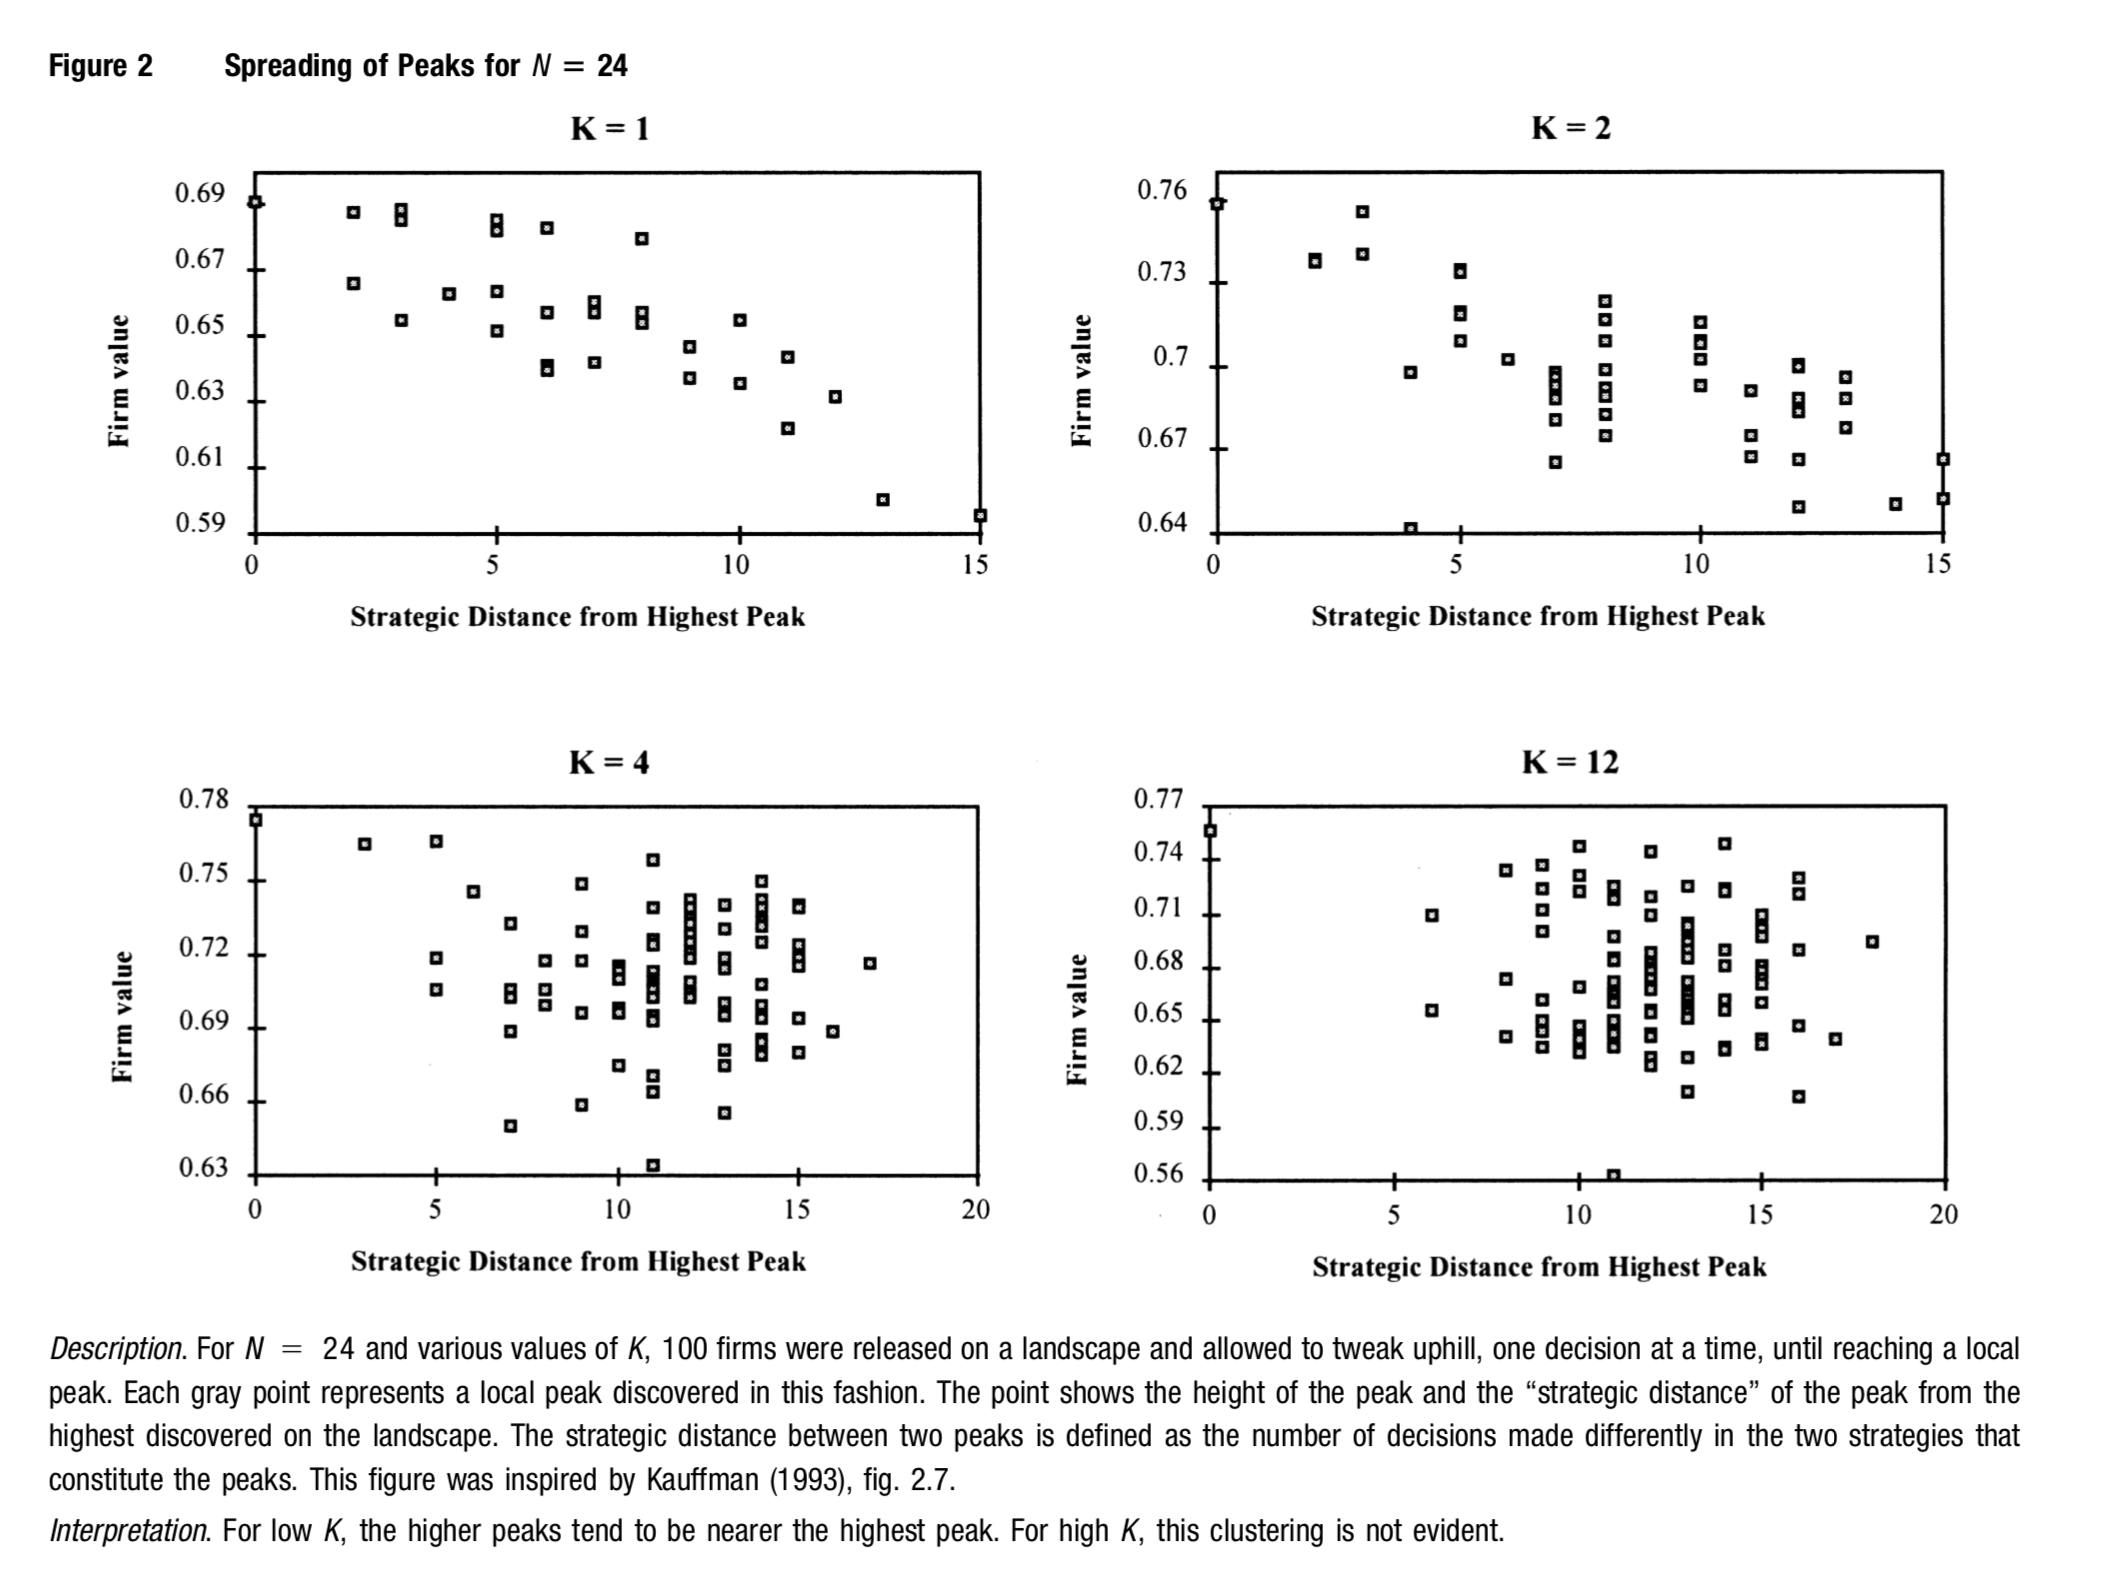
\includegraphics[width=1\textwidth]{Rivkin_Figure.png}
\end{figure}

%%INSERT TABLES
\begin{figure}[h!]
  \caption{Dirichlet Lon}
  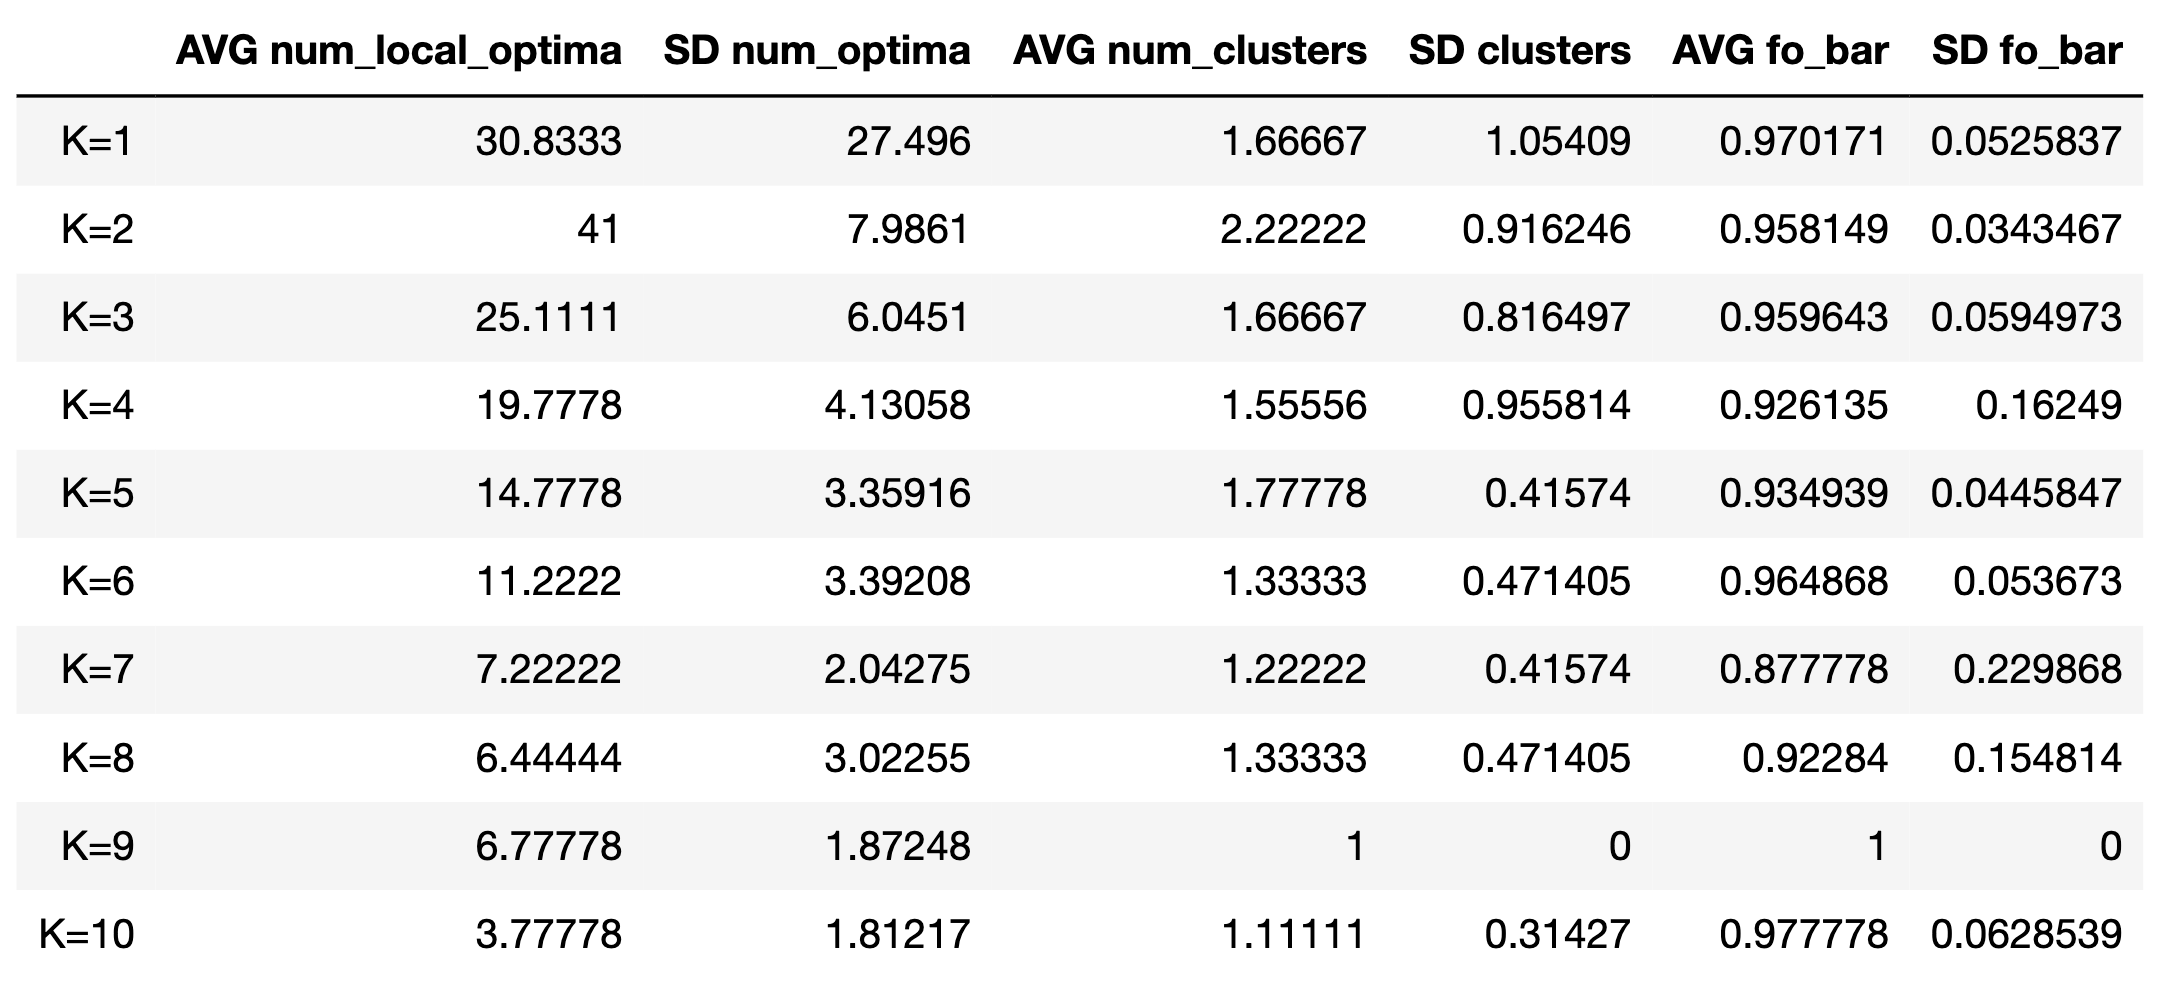
\includegraphics[width=1\textwidth]{Dirichlet_Lon.png}
\end{figure}

%%INSERT TABLES
\begin{figure}[h!]
  \caption{NK Lon}
  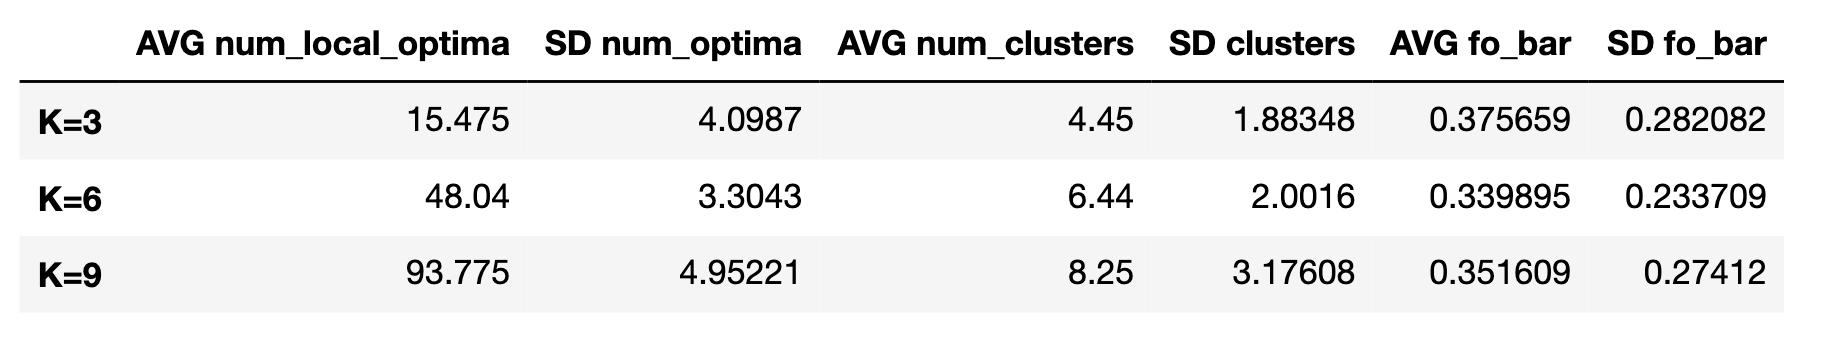
\includegraphics[width=1\textwidth]{NK_Lon.png}
\end{figure}


We may now reconsider some of the past literature in this light. Rivkin (2000) examined how firms may be able to copy strategies from other firms. His key finding was that as a strategy increases in complexity that it will be harder for other firms to copy a strategy. His model assumed that a strategy, a location on a Kauffman N-K landscape, is imperfectly imitated and then firms will make hill-climbing incremental improvements. In this model the copying firms make improvements until they reach a local maxima. We can see his model results in figure 2 copied from his paper below. It is notable to note that as K increases the correlation between the distance from the highest peak and finesses (or firm values) of other reached peaks tends towards zero. This illustrates a property of the Kauffman NK model which the dot model does not imitate, owing to the dot model's higher levels of autocorrelation. Indeed, should a firm make a minor mistake while copying in the standard NK model, disastrous outcomes are likely owing to the low autocorrelation, a global minimum and maximum could be only a few steps away and one may get ensnared in a relatively low local optima traversing between the two.

Indeed the Local Optima Network table illustrates this point most clearly. If one supposes a firm gets stuck while copying and tries to find the global optima by making larger steps, it is more probable in the dot model as the global optima's cluster is large, but no so for the standard NK model. Incremental improvement through somewhat broad search is thus more probable to lead to the global optima in the dot model, and the local optima values one gets stuck in if close to the global optima are likely to not wildly vary from the global optima's value in the dot model.

Some past research has also found that search may be improved by altering a landscape to give it macro-level properties found in the dot model. Gavetti and Levinthal (2000) found that in complex Kauffman landscapes that reducing dimensionality aided in search, however this aid in search arises from the ruggedness in Kauffman landscapes not found in the dot model, and their proposed each strategy is somewhat effective insofar as it does not consider LONs. In their model, representations of a landscape are formed by choosing a subset of N decisions to search over. This representation smooths the landscape as the number of peaks are necessarily reduced. What matters, they write, is that this representation leads to larger basins of attraction; as they cite Kauffman (1993) ``The extent of a basin of attraction is positively correlated with the height of the local peak with which it is associated". That is they find that their method of search through cognitive representations increases the basins of attraction. However for high K, these basins of attraction become negligibly small. Indeed as we have already discussed what matters are the local optima networks. The LONs are essentially basins of attraction, but of a higher step size. In the standard NK the LONs demonstrate that one may become stuck (never reach a global optima) when K is high. Indeed it seems that what Gavetti and Levinthal found is that representations help one shift to a larger basin of attraction, but in essence they are creating a landscape with different properties that allows it to be searched. 

Similar work by Csaszar and Levinthal (2016) similarly illustrated how new landscapes may be created that have better properties for search. However their representation of the landscape (reproduced below) is not properly illustrative of NK models, their model shows a landscape that is rugged in the sense that it has many local peaks, but has the macro property of a clear global optima. In the NK model, when ruggedness is high there is actually little variation with regard to local optima fitness, it more closely resembles the first inverted egg crate model below. Indeed, if anything, Csaszar and Levinthal's model on the left hand side resembles the dot Dirichlet model - a landscape of a form the literature has yet to examine - given the clear existence of a global optima and a gradient of optima finesses that approach it. We further simulated multiple landscapes to identify how far, on average, a location in the top 90th percentile is from the global optima in bit-wise steps; results are graphed below. These clearly illustrate how the dot dirichlet model preserves ``ruggedness" in terms of having local maxima but maintains a steady gradient of optima increasing to the global peak. 


\begin{figure}[h!]
  \caption{Csaszar and Levinthal's Representation}
  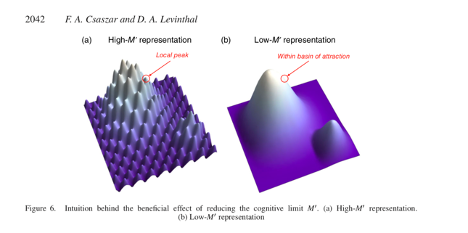
\includegraphics[width=1\textwidth]{Csaszar_Figure.png}
\end{figure}

\begin{figure}[h!]
  \caption{Representation of NK Landscape}
  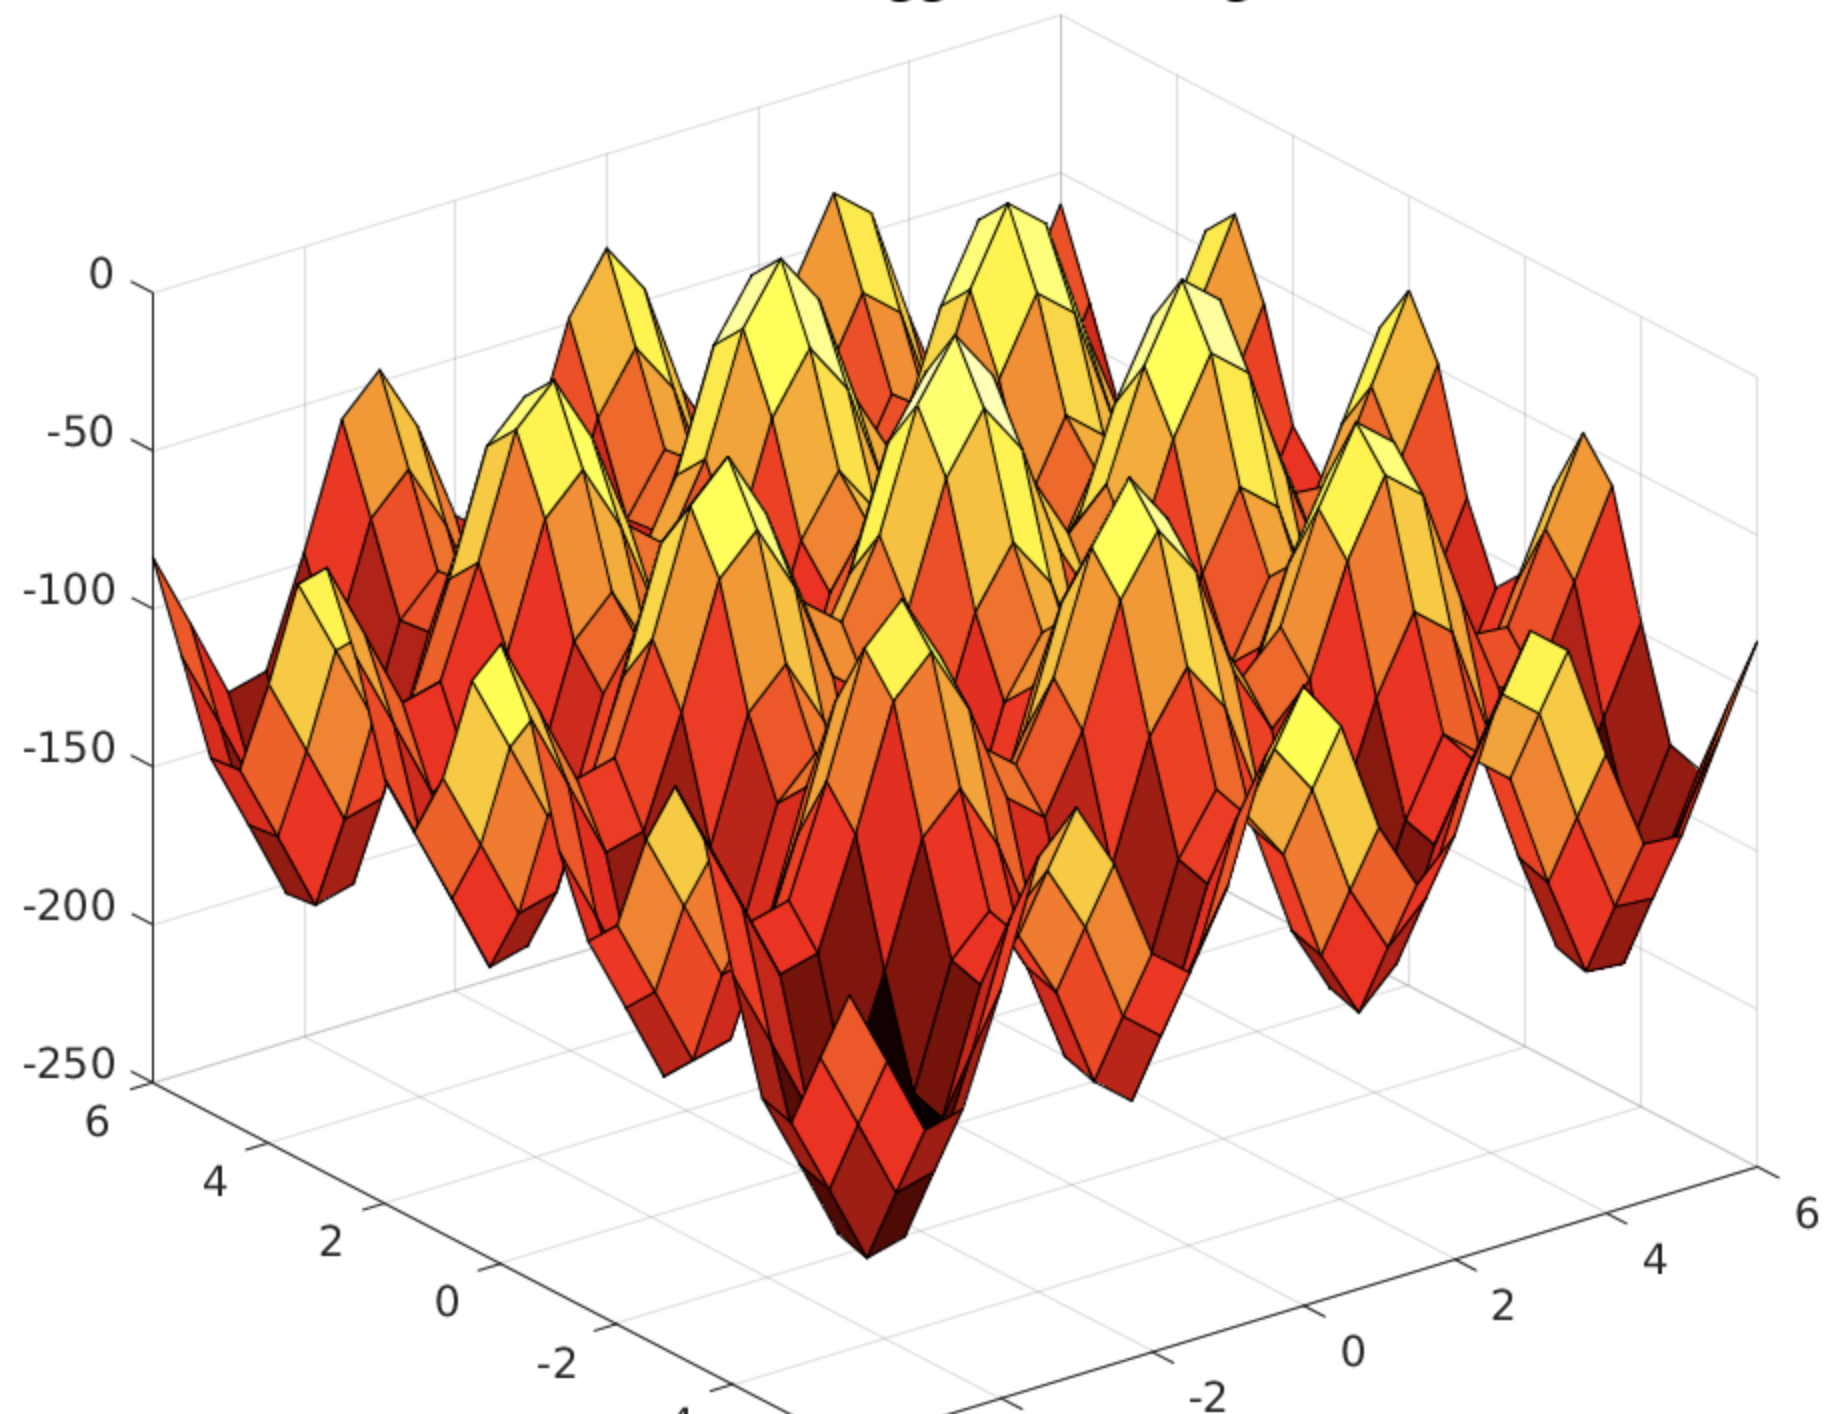
\includegraphics[width=.7\textwidth]{Egg_Crate_Rough.png}
\end{figure}

\begin{figure}[h!]
  \caption{Representation of Dot Dirichlet Landscape}
  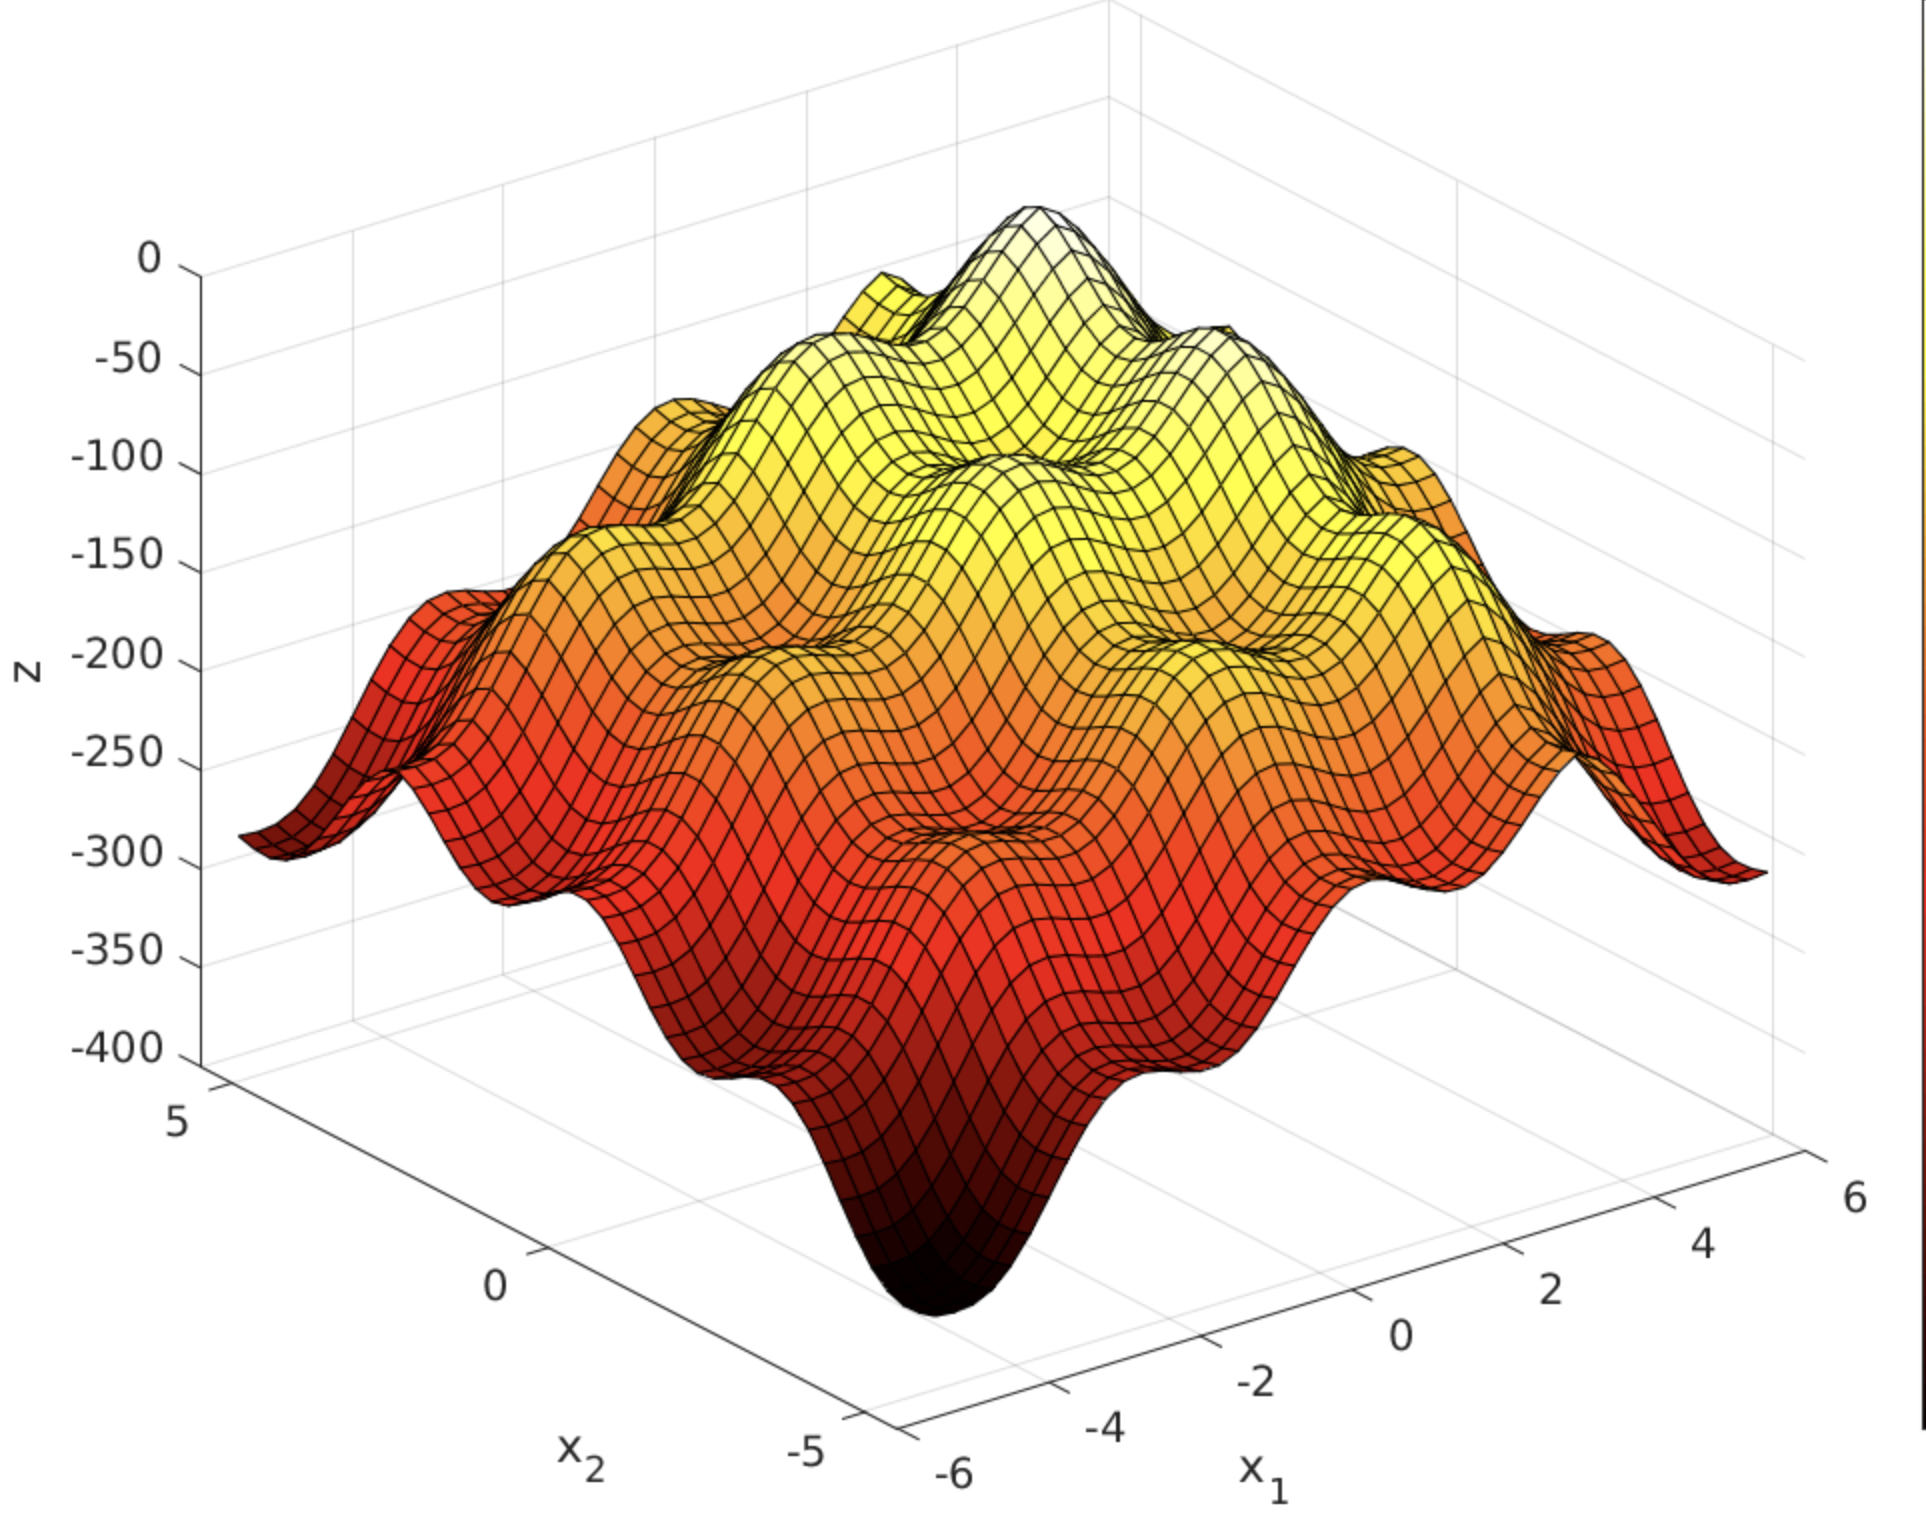
\includegraphics[width=.7\textwidth]{Egg_Crate_Smooth.png}
\end{figure}

\begin{figure}[h!]
  \caption{Distance from 90th percentile to global optimum.}
  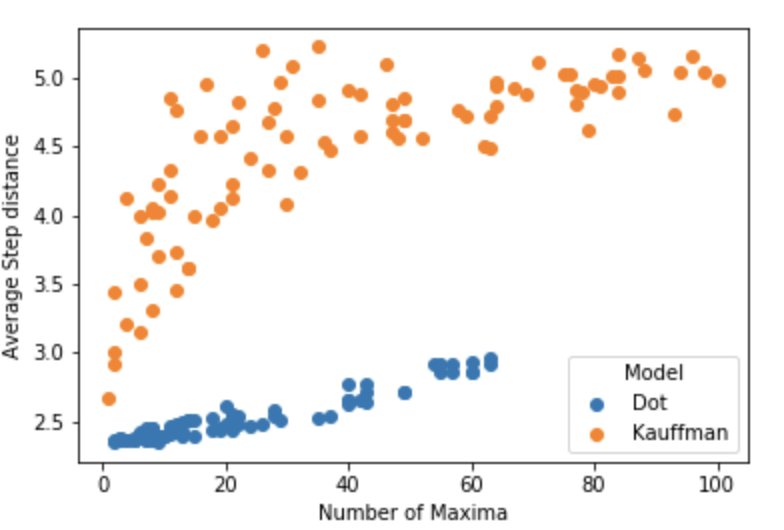
\includegraphics[width=.7\textwidth]{90th_to_Global_Dist.png}
\end{figure}



\end{document}  